\documentclass[aspectratio=169]{beamer}
\usetheme{Berlin}
\usepackage{bookmark}
\usepackage[utf8]{inputenc}
\usepackage[backend=biber]{biblatex}
\addbibresource{./referencie.bib}

\title{Globalización y su impacto en la economía peruana}
\author{Chuquiyauri R. y Palomino A.}
\institute{Universidad Nacional Hermilio Valdizan \\ Facultad de Economía}
\date{2024}

\begin{document}

\begin{frame}
    \begin{columns}
        \column{0.2\textwidth}
            
\includegraphics[width=\textwidth]{./images/unheval.jpg} % Imagen a la izquierda
        \column{0.6\textwidth}
            \titlepage    
        \column{0.2\textwidth}
            
\includegraphics[width=\textwidth]{./images/economia.png} % Imagen a la izquierda
    \end{columns}
\end{frame}

\begin{frame}{\Large Conceptualización de la globalización}
    \begin{columns}
        \column{0.4\textwidth}
            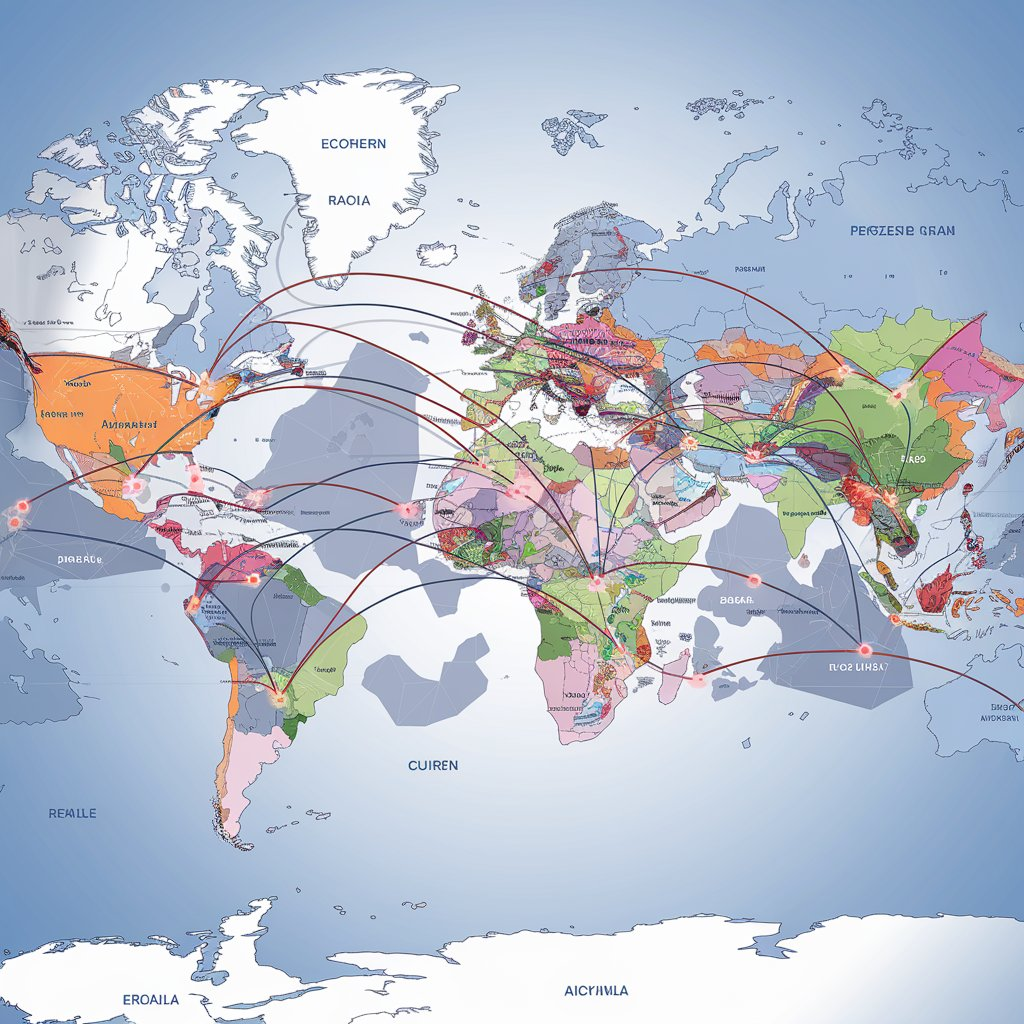
\includegraphics[width=\textwidth]{./images/global.jpeg} % Imagen a la izquierda
        \column{0.6\textwidth}
            \raggedleft % Texto alineado a la derecha
            \Large
            \begin{itemize}
                \item Proceso multidimensional que transforma interacciones económicas, sociales y culturales.
                \item Held y McGrew (2000): redes transnacionales, conciencia global.
                \item Krugman (2018): integración económica con aumento en comercio y movilidad de factores.
            \end{itemize}
    \end{columns}
\end{frame}

\begin{frame}{\Large Contexto histórico en Perú}
    \begin{columns}
        \column{0.6\textwidth}
            \raggedleft % Texto alineado a la derecha
            \Large
            \begin{itemize}
                \item Antecedentes: del período colonial a la apertura en los años 90.
                \item Wise (2003): liberalización, privatización y desregulación de mercados.
                \item Gonzales de Olarte (2015): impacto de reformas estructurales.
            \end{itemize}
        \column{0.4\textwidth}
            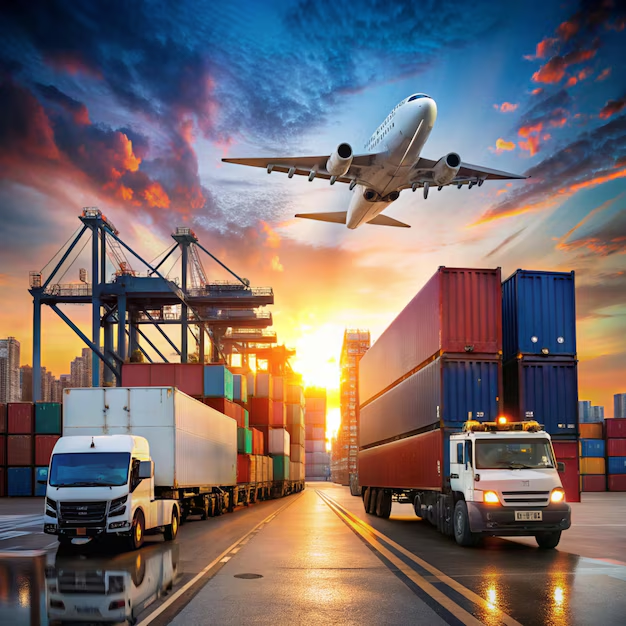
\includegraphics[width=\textwidth]{./images/antecedentes.png} % Imagen a la izquierda
    \end{columns}
\end{frame}

\begin{frame}{\Large Dimensión comercial}
    \begin{columns}
        \column{0.3\textwidth}
            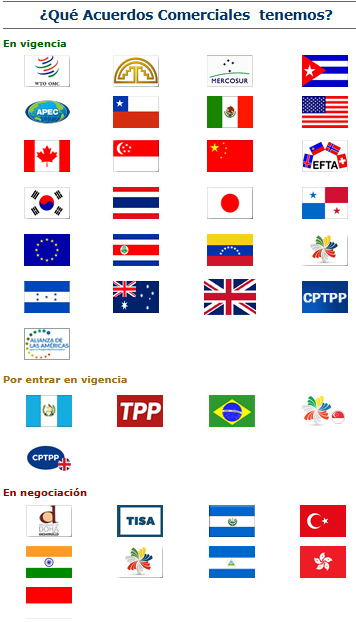
\includegraphics[width=\textwidth]{./images/tlc.png} % Imagen a la izquierda
        \column{0.7\textwidth}
            \raggedleft % Texto alineado a la derecha
            \Large
            \begin{itemize}
                \item Santa Cruz (2021): crecimiento en comercio exterior desde los 90.
                \item TLC: tratados con EE. UU., UE, China, etc.
                \item Ferrero (2018): mayor acceso a mercados, modernización regulatoria.
            \end{itemize}
    \end{columns}
\end{frame}

\begin{frame}{\Large Evolución del comercio exterior}
    \begin{columns}
        \column{0.6\textwidth}
            \raggedleft % Texto alineado a la derecha
            \Large
            \begin{itemize}
                \item Tello (2018): comercio exterior pasó de US\$6.7 mil millones en 1990 a más de US\$98 mil millones en 2019.
                \item Generan cambios interconectados y complejos.
                \item León (2019): diversificación de exportaciones.
            \end{itemize}
        \column{0.4\textwidth}
            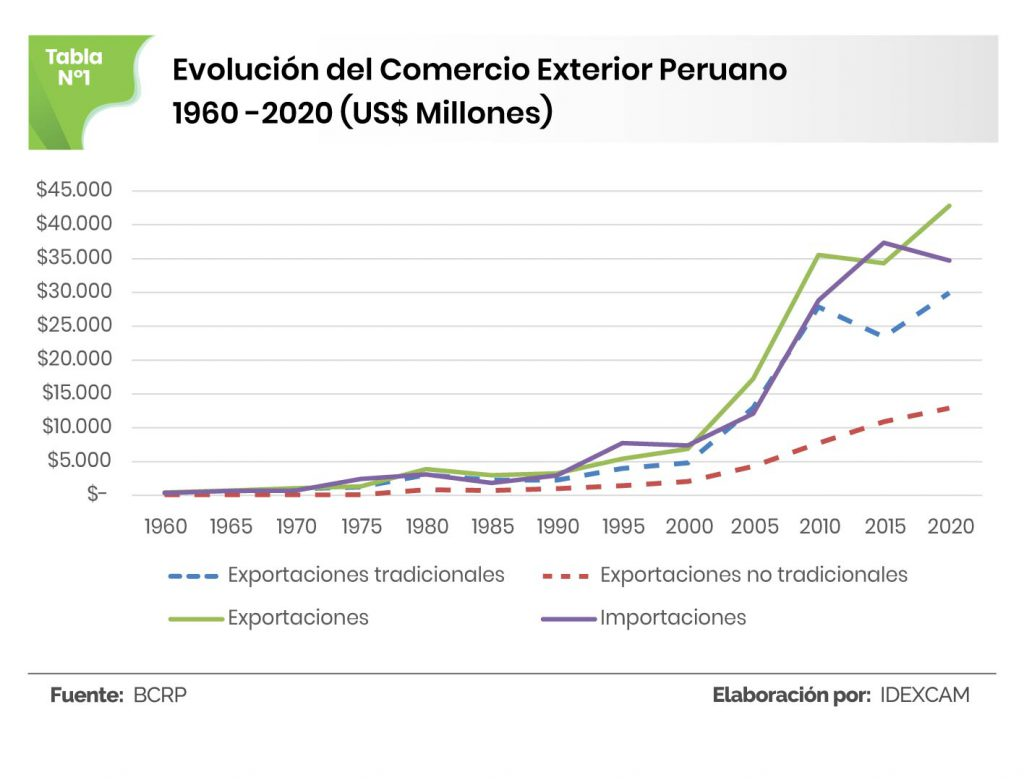
\includegraphics[width=\textwidth]{./images/comercio.png} % Imagen a la izquierda
    \end{columns}
\end{frame}

\begin{frame}{\Large Dimensión productiva}
    \begin{columns}
        \column{0.4\textwidth}
            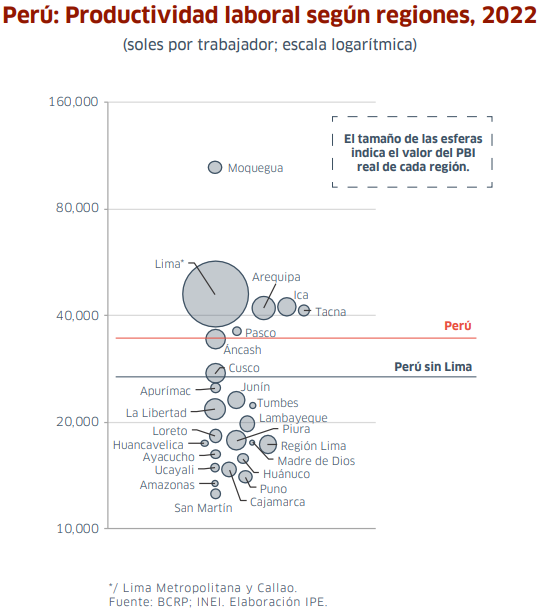
\includegraphics[width=\textwidth]{./images/brecha.png} % Imagen a la izquierda
        \column{0.6 \textwidth}
            \raggedleft % Texto alineado a la derecha
            \Large
            \begin{itemize}
                \item Transformación productiva: reducción del sector industrial, expansión de servicios.
                \item Távara (2020): dualidad productiva, concentrada en Lima y Callao.
                \item Brechas de productividad entre regiones y sectores.
            \end{itemize}
    \end{columns}
\end{frame}

\begin{frame}{\Large Competitividad empresarial}
    \begin{columns}
        \column{0.5\textwidth}
            \raggedleft % Texto alineado a la derecha
            \Large
            \begin{itemize}
                \item Modernización de procesos, certificaciones internacionales.
                \item Torres (2021): integración en cadenas de valor, desafíos de alta informalidad.
                \item Villarreal (2019): barreras de productividad y financiamiento.
            \end{itemize}
        \column{0.5\textwidth}
            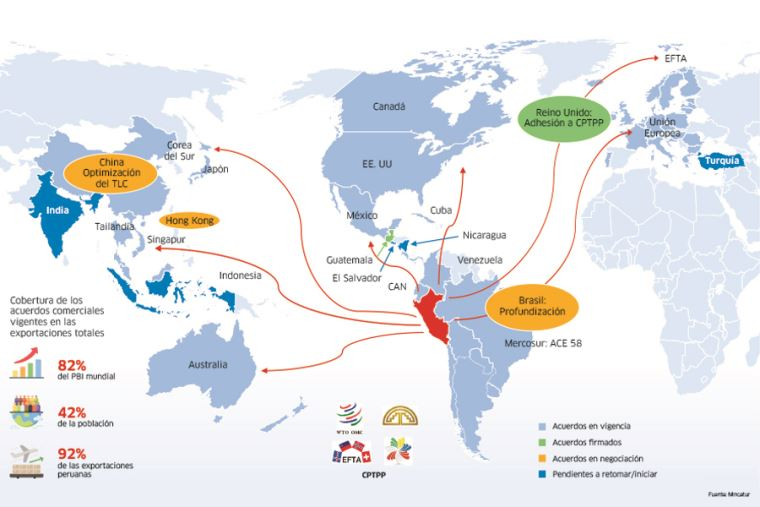
\includegraphics[width=\textwidth]{./images/cgv.png} % Imagen a la izquierda
    \end{columns}

\end{frame}

\begin{frame}{\Large Empleo y mercado laboral}
    \begin{columns}
        \column{0.4\textwidth}
            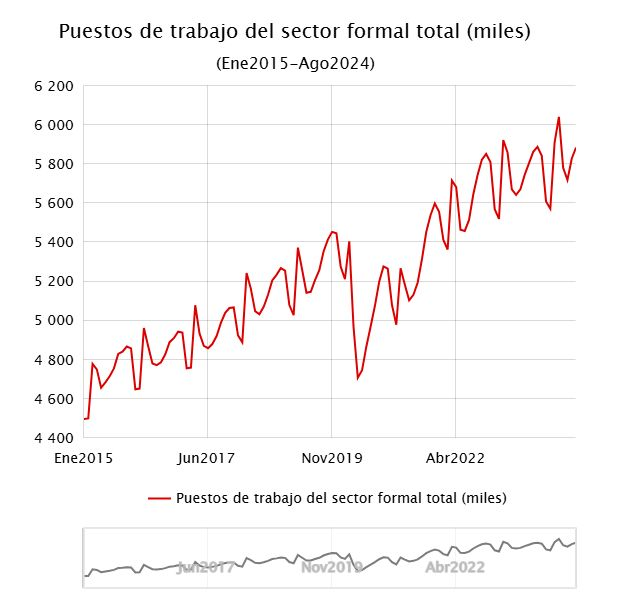
\includegraphics[width=\textwidth]{images/trabajo_formal.jpg}
        \column{0.6\textwidth}
            \Large
            \begin{itemize}
                \item Flexibilización laboral y recomposición de empleo formal.
                \item Chacaltana (2016): crecimiento en comercio formal, pero aumento en temporalidad.
                \item Informalidad persistente (70\% PEA).
            \end{itemize}
    \end{columns}
\end{frame}

\begin{frame}{\Large Distribución del ingreso}
    \begin{columns}
        \column{0.6\textwidth}
            \Large
            \begin{itemize}
                \item Crecimiento reduce pobreza, pero persisten desigualdades.
                \item Webb (2019): pobreza de 58.7\% en 2004 a 20.2\% en 2019.
                \item Mendoza (2020a): desigualdad y rigidez en el coeficiente de Gini.
            \end{itemize}
        \column{0.4\textwidth}
            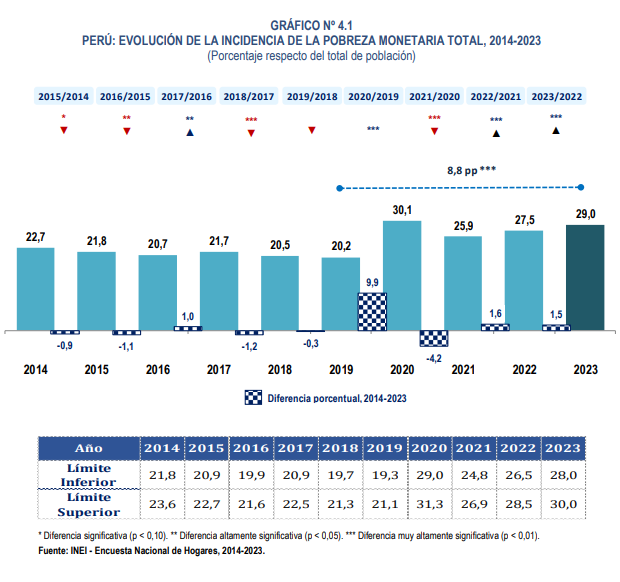
\includegraphics[width=\textwidth]{images/pobreza.png}
    \end{columns}
\end{frame}

\begin{frame}{\Large Desarrollo social}
    \Large
    \begin{itemize}
        \item Mejoras en educación y salud, con brechas entre zonas rurales y urbanas.
        \item Vásquez (2020): aumento de recursos fiscales beneficia acceso a servicios.
        \item Desafíos en la calidad y equidad del acceso a servicios.
    \end{itemize}
\end{frame}

\begin{frame}{\Large Oportunidades económicas}
    \begin{columns}
        \column{0.4\textwidth}
            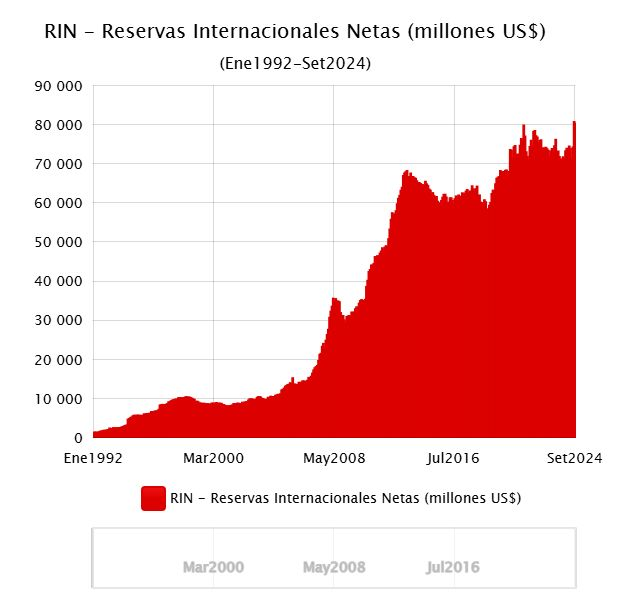
\includegraphics[width=\textwidth]{images/rin.jpg}
        \column{0.6\textwidth}
            \Large
            \begin{itemize}
                \item Crecimiento económico impulsado por el comercio y TLCs.
                \item Dancourt (2018): boom de commodities y diversificación de mercados.
                \item Velarde (2019): estabilidad macroeconómica y acumulación de reservas.
            \end{itemize}

    \end{columns}
\end{frame}

\begin{frame}{\Large Vulnerabilidad y desigualdades sociales}
    \begin{itemize}
        \item Exposición a choques externos y dependencia de commodities.
    \end{itemize}
    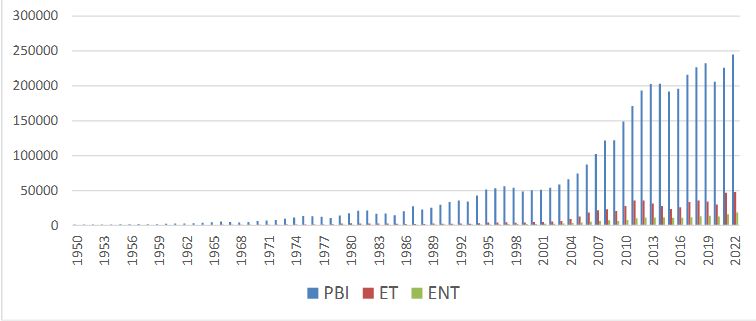
\includegraphics[width=\textwidth]{images/pbi_et_ent.png}
\end{frame}

\begin{frame}{\Large  Sostenibilidad ambiental}
    \Large
    \begin{itemize}
        \item Glave (2021): presión de industrias extractivas sobre recursos naturales.
        \item Vargas (2020): impacto del cambio climático en la agroindustria.
        \item Necesidad de incluir criterios de sostenibilidad en políticas.
    \end{itemize}
\end{frame}

\end{document}
